\documentclass[cn,11pt,chinese]{elegantbook}

\title{基于深度模糊系统的时序数据分析平台}
\subtitle{用户使用手册}

\author{杨腾\& 王元刚}
%\institute{码力无限工作室(Code4Infinity Studio)}
\date{2020年12月20日}
\version{1.0}
%\bioinfo{自定义}{信息}

\extrainfo{封面图片来自pixabay}

%\logo{logo-blue.png}
%\cover{cover1.png}
\cover{cover.jpg}
% 本文档命令
\usepackage{array}
\usepackage{caption}
\usepackage{graphicx}
\usepackage{subfigure}
\usepackage{graphicx}
\newcommand{\ccr}[1]{\makecell{{\color{#1}\rule{1cm}{1cm}}}}

\begin{document}

\maketitle
\frontmatter

%\chapter*{特别声明}
%\markboth{Introduction}{前言}
%
%本文档仅供申请软件著作权使用,未经作者允许,请勿外传或用作其它商业目的,最终解释权归
%
%\underline{如果你无法认同我的想法,建议直接删除本模板。}
%
%\vskip 1.5cm
%
%\begin{flushright}
%Ethan Deng\\
%February 10, 2020
%\end{flushright}

\tableofcontents
%\listofchanges

\mainmatter
\chapter{引言}
\section{背景}
在数据分析领域,时间序列是一类特殊的数据类型,它泛指那些随着时间或空间而发生有序变化的数据。在时间序列中,数据是按照时间的先后顺序来进行排列的观测值。时间序列数据广泛存在于众多应用领域,例如:经济领域的货币汇率、国内总产值;金融工程领域股票、期货的开盘价、收盘价和成交量;环境科学中某地的温度变化,降雨量变化情况;社会领域某学校的入学人数,某车站的人流量等。在实际问题的应用中,随着数据存储和处理能力的不断提升,数据能够被长期储存,这使得在许多应用领域中数据更多地被存储为时间序列的形式。对于获得的时间序列数据,如何通过充分且有效地管理和分析,以挖掘、捕获时间序列所隐含的规律和特性,并能够用于处理实际问题是十分重要的研究方向,该方面的研究已经受到越来越多研究者的关注,时间序列分析也随之产生。

时间序列广泛存在于包含时间度量的各应用科学领域,时间序列分析是通过对时间序列进行研究来挖掘序列的特性以及序列中存在的有意义的规律,能够提炼出有价值的信息用以进一步的应用。时间序列分析的研究任务包括时间序列分割、预测、匹配、异常检测、聚类、分类、可视化和趋势分析等,其中时间序列预测是该领域最常见也是最有应用潜力的问题之一。时间序列预测是指根据现有的观测值,通过建立模型或者寻找规则,给出未发生数据的预测值。在建立模型或寻找规则的过程中,需要对时间序列存在的规律进行科学、理性地认识,预测是对建立的模型最直接的应用。根据预测的步数,可将时间序列预测问题分为一步预测、多步预测和长期预测。时间序列预测能够在一定程度上帮助决策者规避风险,以便进行更有利的决策。

\section{目的和意义}


\section{参考资料}


\chapter{开发工具与环境}


\section{开发工具}

本平台的开发工具主要使用的编程语言是Python,开发工具选用PyCharm,开发框架使用PyQt5,算法使用Numpy实现,作图使用Matplotlib。

PyCharm是用于Python脚本语言的最流行的IDE,具有跨平台性,为用户和开发人员在代码完成和检查,高级调试和支持Web编程框架等方面提供了最好的功能。在编写Python时,无论是内置还是外置软件包,PyCharm均可实现更流畅的包和模块的引用。SQLAlchemy作为调试器可以设置断点,在调试器中暂停,并可以查看用于SQL语言代码的用户表达式的SQL表示。编辑器中Git可以可视化,这在Python中编码时,对团队开发提供了有利的支持,开发人员可以在PyCharm中轻松检查上次提交的内容,因为PyCharm具有可以定义上次提交与当前提交之间的区别的部分。PyCharm专业版可以在External Tools中配置QtDesigner,对开发图形界面有较好的交互式功能。另外,PyCharm对Python项目代码重构也有较好的支持,每一次修改的内容会广播到整个项目的所有引用到此修改内容的位置,进而节省了大量时间。

QyQt5是一套Python绑定Digia QT5应用的框架。它可用于Python 2和3。Qt是一组跨平台c++库,它们实现了高级的api,用于访问现代Windows桌面和移动系统的许多方面。其中包括定位服务、多媒体、NFC和蓝牙连接、基于Chromium的web浏览器,以及传统的UI开发。PyQt5实现为超过35个扩展模块,620多个类和6000个函数和方法。它是一个跨平台的工具包,它可以运行在所有主要的操作系统,包括UNIX,Windows,MacOS。PyQt5是双重许可,开发者可以在GPL和商业许可之间进行选择。PyQt5还可以嵌入到基于c++的应用程序中,以允许这些应用程序的用户配置或增强这些应用程序的功能。PyQt5的类别分为几个模块,包括以下:

\begin{itemize}
\item QtCore:包含了核心的非GUI功能。此模块用于处理时间、文件和目录、各种数据类型、流、URL、MIME类型、线程或进程。
\item QtGui:包含类窗口系统集成、事件处理、二维图形、基本成像、字体和文本。
\item QtWidgets:模块包含创造经典桌面风格的用户界面提供了一套UI元素的类。
\item QtMultimedia:包含的类来处理多媒体内容和API来访问相机和收音机的功能。
\item QtBluetooth:模块包含类的扫描设备和连接并与他们互动。描述模块包含了网络编程的类。这些类便于TCP和IP和UDP客户端和服务器的编码,使网络编程更容易和更便携。
\item QtNetwork:QNetworkProxy类提供了一个网络层代理。
\item QtPositioning:包含类的利用各种可能的来源,确定位置,包括卫星、Wi-Fi、或一个文本文件。
\item Enginio:模块实现了客户端库访问Qt云服务托管的应用程序运行时。
\item QtWebSockets:模块包含实现WebSocket协议类。
\item QtWebKit:包含一个基于Webkit2图书馆Web浏览器实现类。
\item QtWebKitWidgets:包含的类的基础webkit1一用于qtwidgets应用Web浏览器的实现。
\item QtXml:包含与XML文件的类。这个模块为SAX和DOM API提供了实现。
\item QtSvg:模块提供了显示SVG文件内容的类。可伸缩矢量图形(SVG)是一种描述二维图形和图形应用的语言。
\item QtSql:模块提供操作数据库的类。
\item QtTest:包含的功能,使pyqt5应用程序的单元测试
\end{itemize}
~\\

本平台主要使用了Python版本的PyQt5,用到的组件有:QTabWidget、QTextEdit、QLabel、QLineEdit、QPushButton、QMessageBox、QTableWidget,主面板使用水平布局 QHBoxLayout,子面板全部使用网格布局 QGridLayout。
~\\

\begin{itemize}
\item QWidget:QWidget类是所有用户界面对象的基类,被称为基础窗口部件。像主窗口、对话框、标签、还有按钮、文本输入框等都是窗口部件。这些部件可以接受用户输入,显示数据和状态信息,并且在屏幕上绘制自己。
\item QTabWidget:QTabWidget控件提供了一个选项卡和一个页面区域,默认显示第一个选项卡的页面,通过单击各选项卡可以查看对应的界面,如果在一个窗口中显示的输入字段很多,则可以对这些字段进行拆分,分别放置在不同界面的选项卡中。
\item QTextEdit:QTextEdit类是一个多行文本框控件,可以显示多行文本内容,当文本内容超出控件显示范围时,可以显示水平个垂直滚动条,Qtextedit不仅可以用来显示文本还可以用来显示HTML文档。
\item QLabel:QLabel的作用包括占位符、显示文本、显示图片、放置gif动画、超链接、提示标记。
\item QLineEdit:就是QTextEdit的单行形式。使用者可以通过很多函数,输入和编辑单行文本,比如撤销、恢复、剪切、粘贴以及拖放等。
\item QPushButton:QAbstractButton类为抽象类,不能实例化,必须由其他的按钮类继承QAbstractButton类,来实现不同的功能和表现形式,常见的按钮QPushButton,QToolButton,QRadioButton和QCheckBox这些按钮均继承自QAbstractButton类,根据各自的使用场景通过图形显示出来。
\item QMessageBox:QmessageBox是一种通用的弹出式对话框,用于显示消息,允许用户通过单击不同的标准按钮对消息进行反馈,每个标准按钮有一个预定义的文本,角色和十六进制数,QMessageBox类提供了许多常用的弹出式对话框,如提示。警告,错误,询问,关于,等会话框,这些不同类型的QMessageBox对话框只是显示的图标不同,其他的功能是一样的。
\item QTableWidget:QTableWidget是Qt程序中常用的显示数据表格的控件,类似于c\# 中的DataGrid。QTableWidget是QTableView的子类,它使用标准的数据模型,并且其单元数据是通过QTableWidgetItem对象来实现的,使用QTableWidget时就需要 QTableWidgetItem。用来表示表格中的一个单元格,整个表格就是用各个单元格构建起来的。
\item QHBoxLayout:采用QBOXLayout类可以在水平和垂直方向上排列控件,QHBoxLayout 和 QVBoxLayout类继承自QBoxLayout。采用QHBoxLayout类,按照从左到右的顺序来添加控件。
\item QGridLayout:QGridLayout(网格布局)是将窗口分割成行和列的网格来进行排列,通常可以使用函数addWidget将被管理的控件(Widget)添加到窗口中,或者使用addLayout函数将布局(layout)添加到窗口中,也可以通过addWIdget函数对所添加的控件设置行数与列数的跨越,最后实现网格占据多个窗格。
\item QFormLayout:QFormLayout是label-field式的表单布局,顾明思议,就是实现表单方式的布局,表单是提示用户进行交互的一种模式,主要有两列组成,第一列用于显示信息,给用户提示,一般叫做label域,第二列需要用户进行选择或输入,一般叫做field域,label与field的关系就是label关联field。
\item QPixmap:QPixmap类用于绘图设备的图像显示,它可以作为一个QPainterDevice对象,也可以加载到一个控件中,通常是标签或者按钮,用于在标签或按钮上显示图像。QPixmap可以读取的图像文件类型有BMP,GIF,JPG等格式。
\end{itemize}
~\\

Numpy(Numerical Python)是 Python 语言的一个扩展程序库,支持大量的维度数组与矩阵运算,此外也针对数组运算提供大量的数学函数库,机器学习算法中大部分都是调用Numpy库来完成基础数值计算的。NumPy 是一个运行速度非常快的数学库,主要用于数组计算,它的功能包括一个强大的N维数组对象ndarray、广播功能函数、整合 C/C++/Fortran 代码的工具、线性代数、傅里叶变换、随机数生成等功能。Numpy 通常与 Scipy(Scientific Python)和 Matplotlib(绘图库)一起使用, 这种组合广泛用于替代 MatLab,MatLab是一个强大的科学计算环境,有助于我们通过 Python 学习数据科学或者机器学习。在编写机器学习算法时,需要对矩阵进行各种数值计算,例如矩阵乘法、换位、加法等。NumPy数组用于存储训练数据和机器学习模型的参数。计算机中的图像表示为多维数字数组,因此NumPy成为同样情况下最自然的选择。实际上,NumPy提供了一些优秀的库函数来快速处理图像。例如,镜像图像、按特定角度旋转图像等。在NumPy中维度(dimensions)叫做轴(axes),轴的个数叫做秩(rank)。NumPy对于执行各种数学任务非常有用,如数值积分、微分、内插、外推等。因此,当涉及到数学任务时,它形成了一种基于Python的MATLAB的快速替代。

Matplotlib 是一个 Python 的 2D绘图库,它以各种硬拷贝格式和跨平台的交互式环境生成出版质量级别的图形。Matplotlib可以帮助我们绘制线图、散点图、等高线图、条形图、柱状图、3D 图形、甚至是图形动画等等。为了简单绘图,它的 pyplot 模块提供了类似于MATLAB的界面,尤其是与IPython结合使用时。 对于高级用户,您可以通过面向对象的界面或MATLAB用户熟悉的一组功能来完全控制线型,字体属性,轴属性等。

\section{开发环境}

本平台的软件环境如下:

\begin{itemize}
	\item PyCharm:PyCharm 2020.2.5 (Community Edition)
	\item PyDev Console: IPython 7.19.0
	\item Python版本:Python 3.8.6
	\item PyQt: PyQt 5.12.3
	\item Matplotlib:Matplotlib 3.3.2
	\item Numpy: Numpy 1.18.5
	\item Tqdm : tqdm 4.51.0
	\item Joblib: joblib 0.17.0
	\item Sklearn: scikit-learn 0.23.2
\end{itemize}

(1)ipython是一个python的交互式shell,比默认的python shell好用得多,支持变量自动补全,自动缩进,支持bash shell命令,内置了许多很有用的功能和函数。它也是利用Python进行科学计算和交互可视化的一个最佳的平台,在开发时可以实时监控数据的格式类型和数据的传递方式。

(2)有时候在使用Python处理比较耗时操作的时候,为了便于观察处理进度,就需要通过进度条将处理情况进行可视化展示,以便我们能够及时了解情况。Tqdm是一个快速,可扩展的Python进度条,可以在 Python 长循环中添加一个进度提示信息,用户只需要封装任意的迭代器 tqdm(iterator)。Tqdm可以实时输出处理进度而且占用的CPU资源非常少,支持windows、Linux、mac等系统,支持循环处理、多进程、递归处理、还可以结合linux的命令来查看处理情况,等进度展示。

(3)scikit-learn 是基于 Python 语言的机器学习工具,scikit-learn的metrics库内包含了大量的回归模型的评估方法。在训练和预测阶段需要计算RMSE(均方误差根),使用scikit-learn库中metrics里的mean\_squared\_error计算均方误差,再计算均方误差的算术平方根得到RMSE。

(4)Joblib是一组用于在Python中提供轻量级流水线的工具。它的特点是拥有透明的磁盘缓存功能和惰性的重新评估模式(memoize模式),且适合简单的并行计算,因此Joblib可以将模型保存到磁盘并可在必要时重新运行。相比于Pickle,Joblib适合大数据量的模型,且只能往硬盘存储,不能往字符串存储。


\section{运行环境}

本平台的运行环境如下:

\begin{itemize}
	\item 操作系统:Windows 10.20H(x64)
	\item 计算机内存:8G
	\item 计算机CPU:Intel(R) Core(TM) i5-7500CPU 3.40GHz 3.41GHz
	\item 计算机存储空间:1T
	\item 计算机显卡:Intel(R) HD Graphics 630
	\item PC显示器分辨率:1920 *1080
\end{itemize}

\chapter{模块的设计与功能}

本平台的主模块由两部分组成,数据部分和控制台部分。平台界面默认显示在显示器的屏幕中央,界面的高为屏幕分辨率的65\%,宽为屏幕分辨率的50\%,平台logo选用的阿里巴巴矢量图标库中的时间序列预测logo。

\begin{itemize}
	\item 控制台部分是一个Python Console 用于获取控制台的打印信息,控制台由QTextEdit组件设计实现,平台运行时在IDLE输出的信息都将实时打印在控制台里,如图\ref{main_data}。
	
	\item 数据部分由五个可切换的选项卡构成,分别为数据读取模块、数据处理模块、参数设置模块、模型训练模块和模型测试模块。选项卡是通过QTabWidget设计的,每个选项卡都是一个QWidget,QWidget里用来设计每个选项卡的各种组件和功能,如图\ref{main_console}。
\end{itemize}

\begin{figure}
	\centering
	\subfigure[数据部分]{
		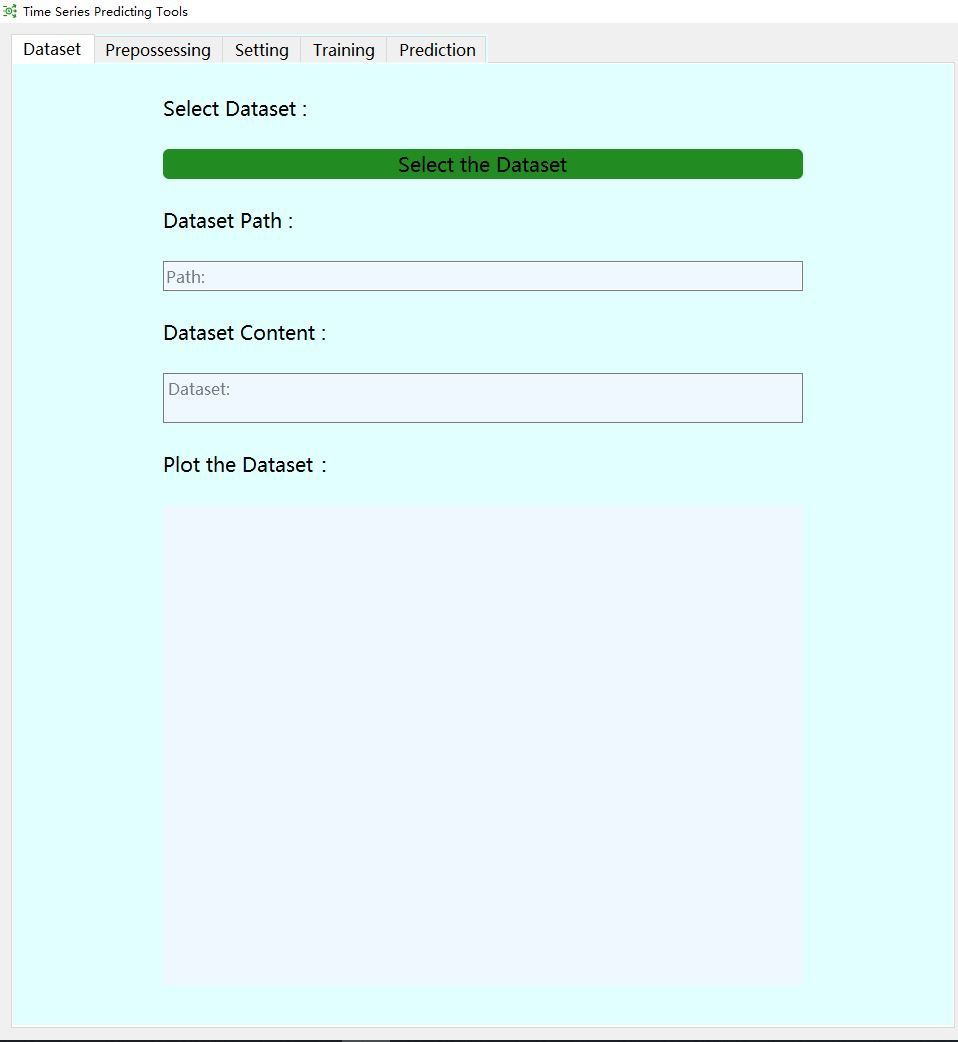
\includegraphics[width = 0.48\textwidth]{figure//main_2.jpg}\label{main_data}
	}
	\subfigure[控制台部分]{
		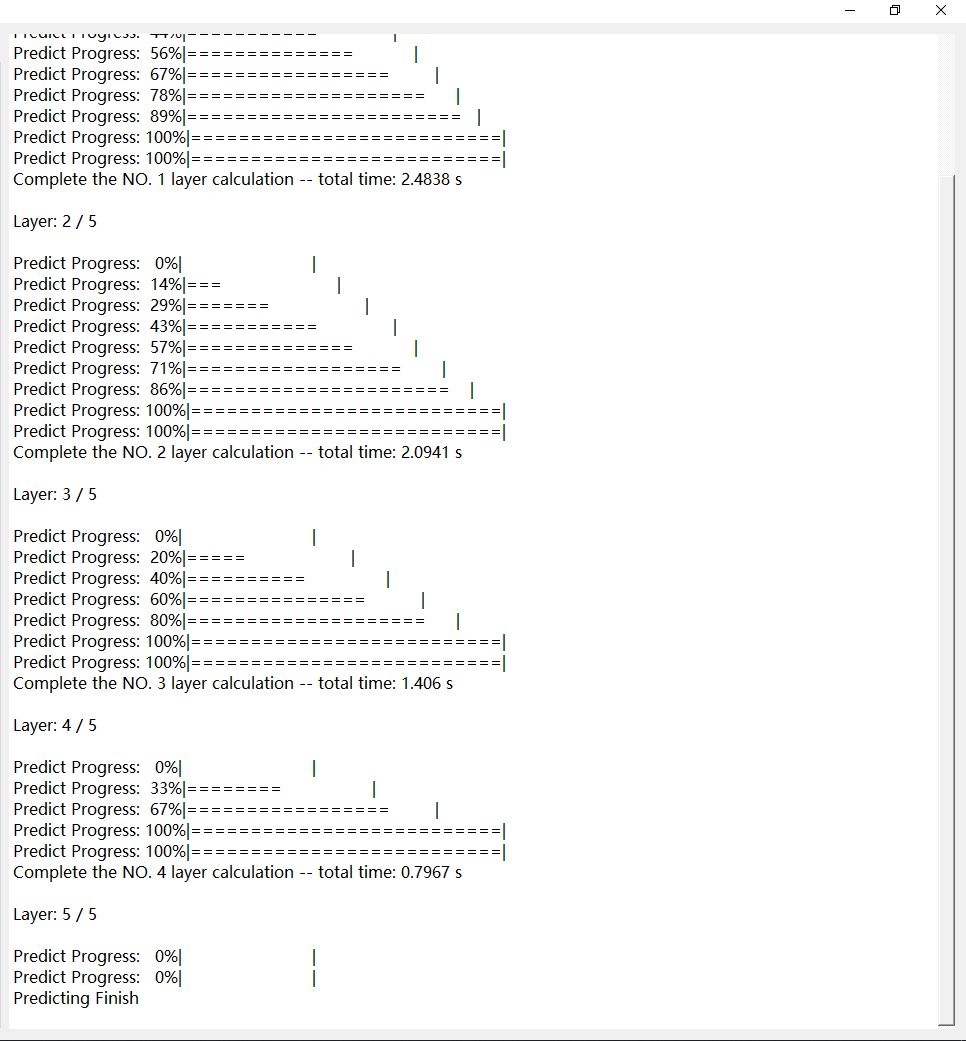
\includegraphics[width = 0.48\textwidth]{figure//main_3.jpg}\label{main_console} 
	}\\
	\caption{主面板的两个部分}
	\label{main_window}
\end{figure}

\section{数据读取模块}

数据读取模块采用网格布局,它的整体是一个QWidget窗口组件,宽高均为自适应。该模块由四个部分组成,分别是时间序列数据集文件的选择按钮,数据集的本地路径显示框,时间序列原始数据的显示框和序列原始数据集展示区域框,每个组件都有与其对应的标签,路径显示框和数据集显示框均设置为不可编辑,按钮可重复单击,如图\ref{load_1}。

\begin{figure}
	\centering
	\subfigure[数据读取模块]{
		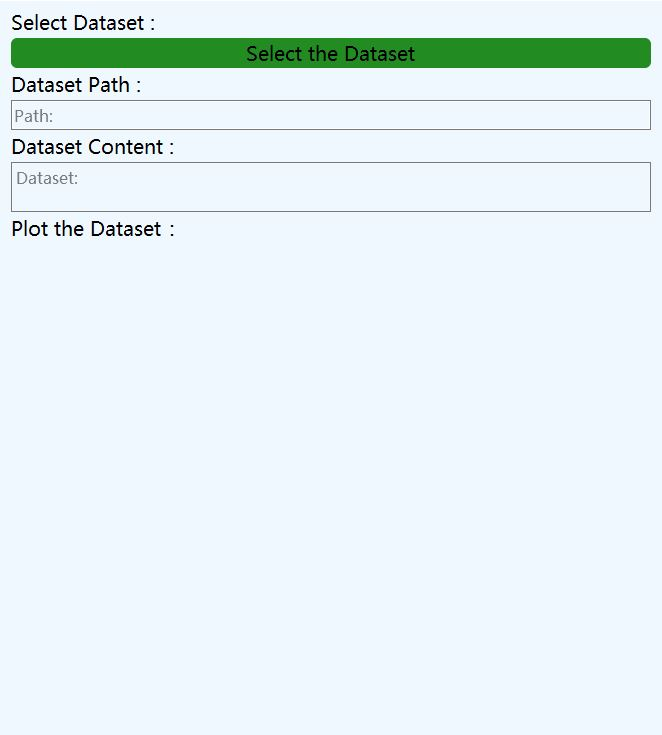
\includegraphics[width = 0.48\textwidth]{figure//load_1.jpg}\label{load_1}
	}
	\subfigure[数据文件选择操作]{
		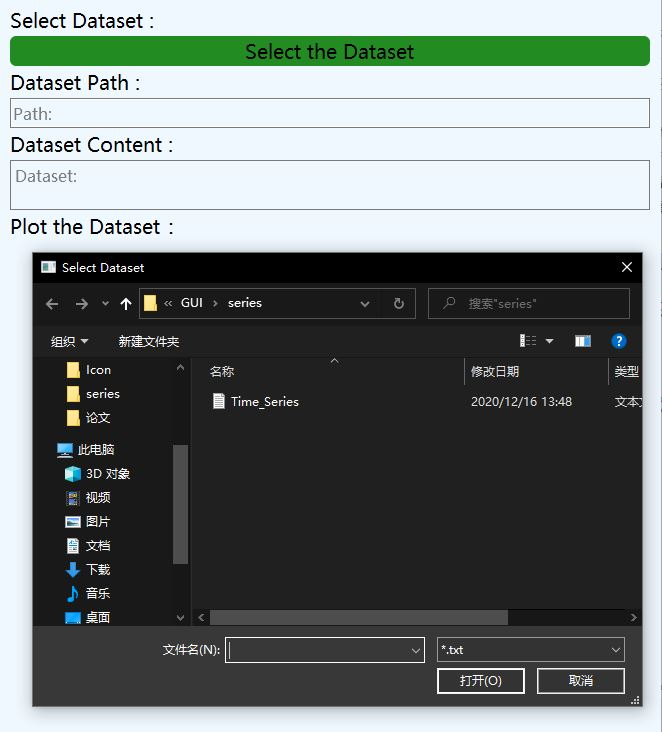
\includegraphics[width = 0.48\textwidth]{figure//load_2.jpg}\label{load_2} 
	}
	\subfigure[数据路径和原始数据内容]{
		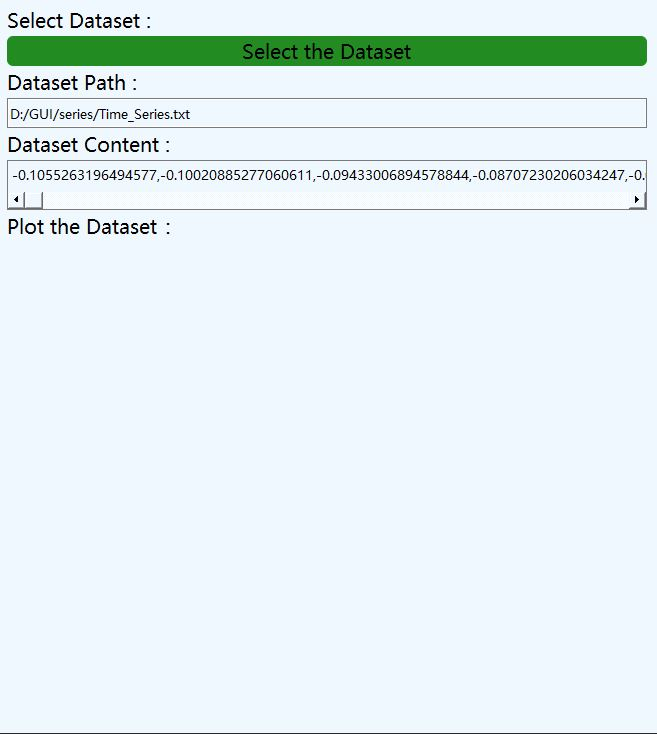
\includegraphics[width = 0.48\textwidth]{figure//load_3.jpg}\label{load_3} 
	}
	\subfigure[原始数据作图]{
		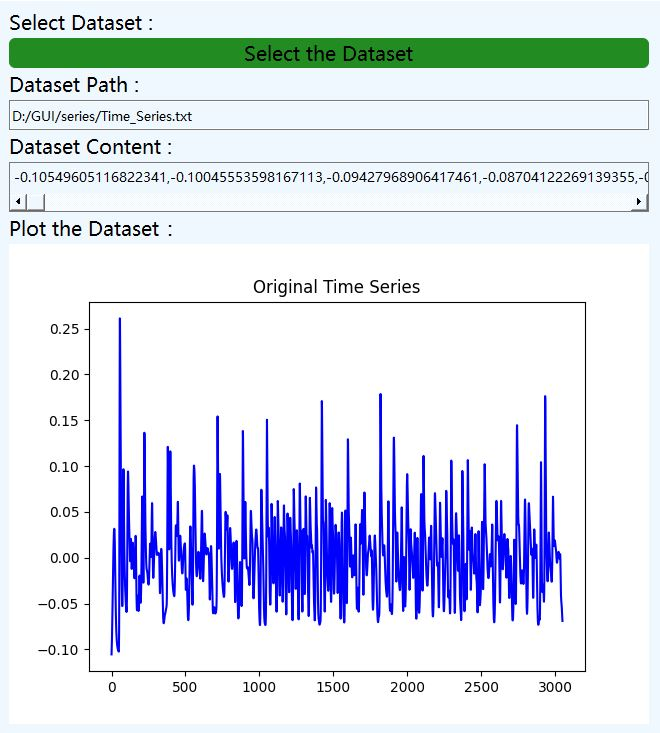
\includegraphics[width = 0.48\textwidth]{figure//load_4.jpg}\label{load_4} 
	}\\
	\caption{数据读取模块操作}
	\label{load}
\end{figure}

\begin{itemize}
	\item 文件选择按钮:文件选择按钮由QPushButton组件实现。该按钮的功能是单击按钮后弹出文件选择框,默认打开的路径为项目的根目录中的series文件夹,如图\ref{load_2},文件夹存放的是txt格式的时间序列文件,按钮已设置成只可以打开txt格式的数据文件,选中要打开的文件后单击打开完成时间序列数据集选择操作。
	\item 路径显示框:路径显示框由QLineEdit组件实现。该文本框为单行显示,用于显示按钮事件返回的数据文件的绝对路径,如图\ref{load_3}。
	\item 数据集显示框:数据集显示框由QTextEdit组件实现。该文本框为多行显示,但因时间序列数据集的特殊性,将他设置成单行显示且不换行,且横向显示滚动条,通过拉伸滚动条可以查看完整的序列数据,如图\ref{load_3}。
	\item 数据作图展示框:作图展示框的底层由Qlabel实现,图像显示在QPixmap组件上,QPixmap可以在代码中对读取的图片尺寸进行放缩,如图\ref{load_4}。
\end{itemize}

\section{数据处理模块}

数据处理模块使用网格布局QGridLayout,它的整体是一个QWidget窗口组件,宽高均为自适应。该模块由五个部分组成,分别是时间序列周期输入框,数据集处理按钮,处理后的时间序列数据表,处理后数据保存路径显示框和数据集保存按钮。其中周期需要用户手动输入,处理后数据保存路径显示框不可编辑,按钮可重复单击,如图\ref{deal_1}

\begin{figure}
	\centering
	\subfigure[数据处理模块]{
		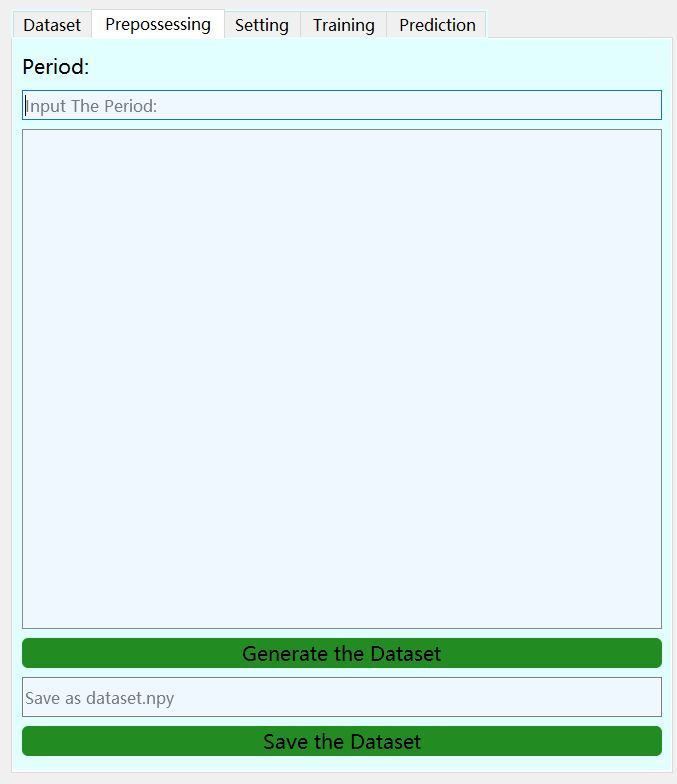
\includegraphics[width = 0.48\textwidth]{figure//deal_1.jpg}\label{deal_1}
	}
	\subfigure[时间序列周期输入]{
		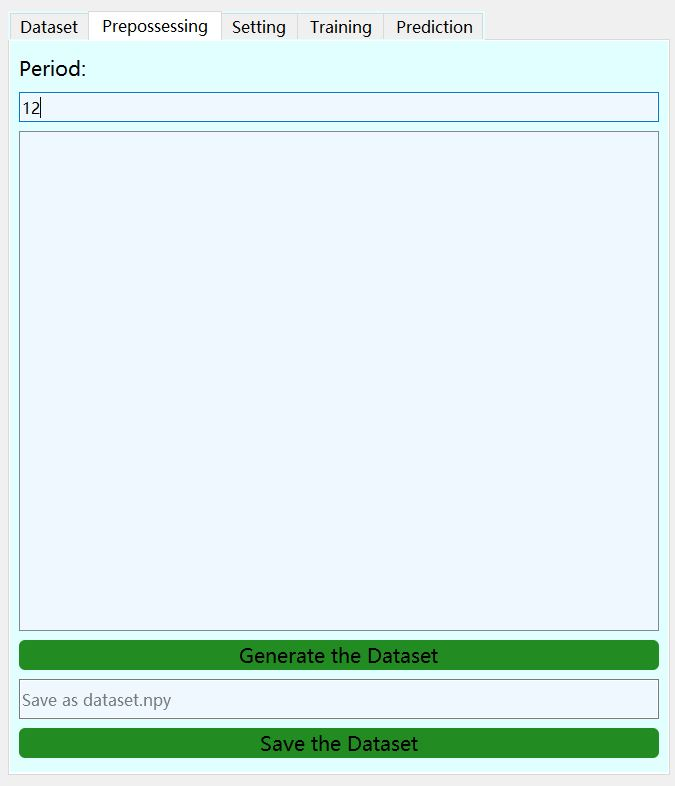
\includegraphics[width = 0.48\textwidth]{figure//deal_2.jpg}\label{deal_2} 
	}
	\subfigure[生成处理后的数据表]{
		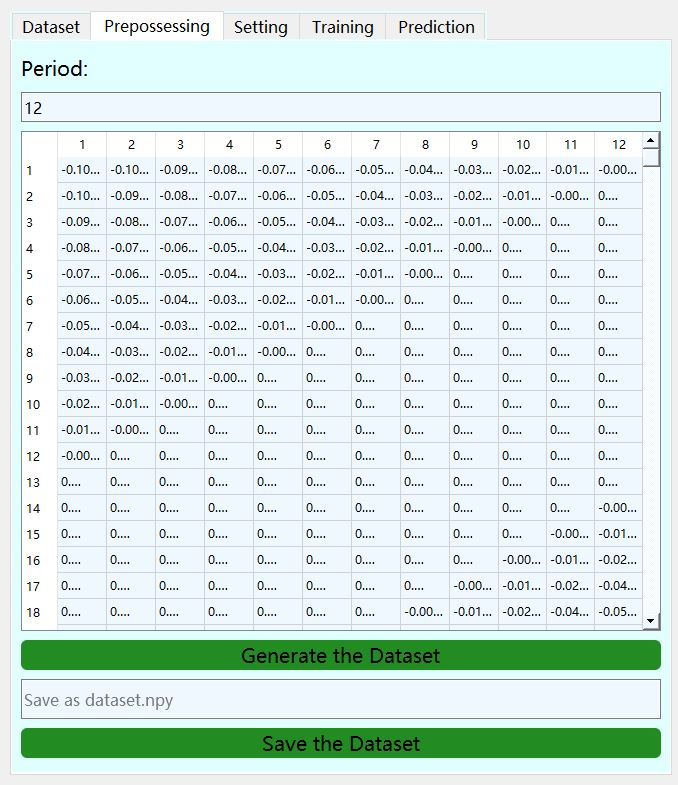
\includegraphics[width = 0.48\textwidth]{figure//deal_3.jpg}\label{deal_3} 
	}
	\subfigure[保存数据表]{
		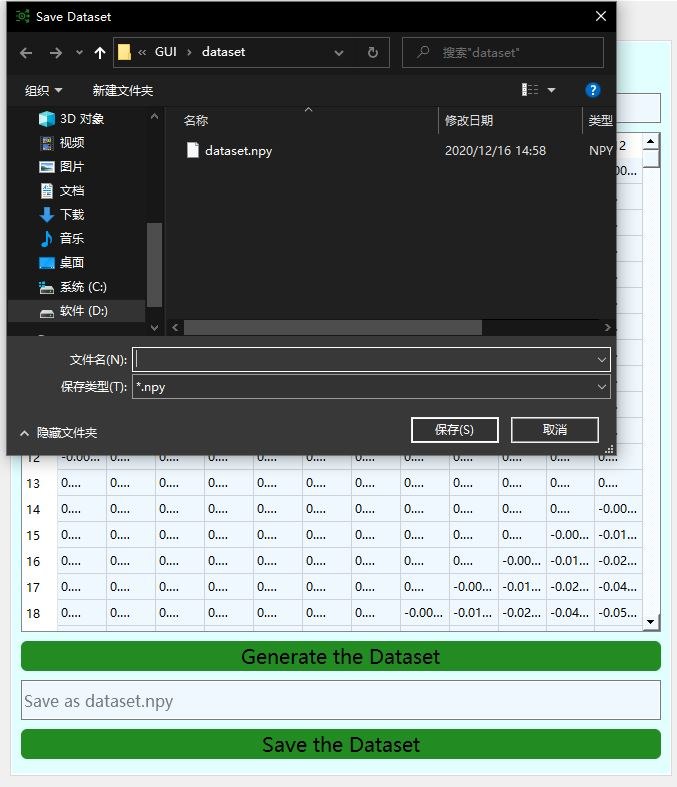
\includegraphics[width = 0.48\textwidth]{figure//deal_4.jpg}\label{deal_4} 
	}
	\subfigure[选择保存路径]{
		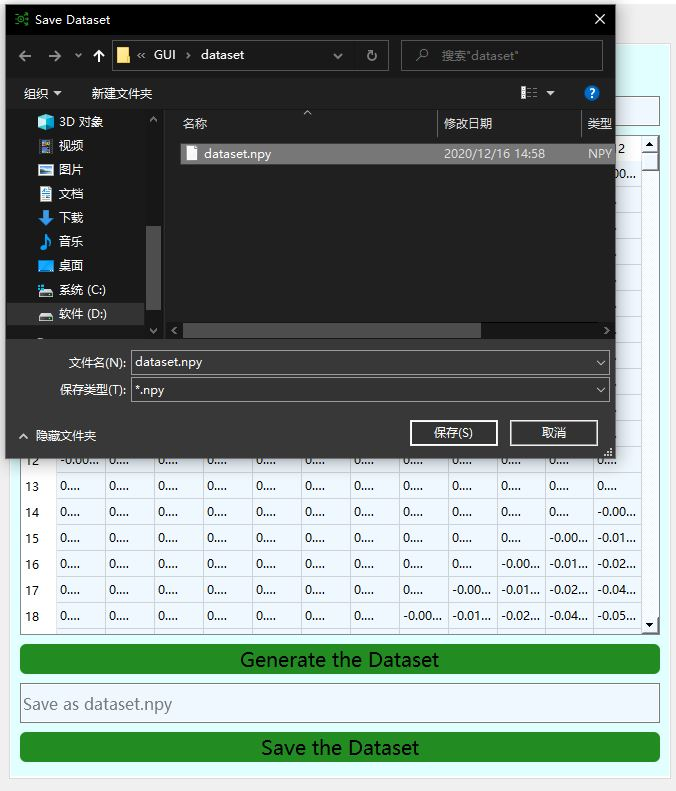
\includegraphics[width = 0.48\textwidth]{figure//deal_5.jpg}\label{deal_5} 
	}
	\subfigure[数据表保存完毕]{
		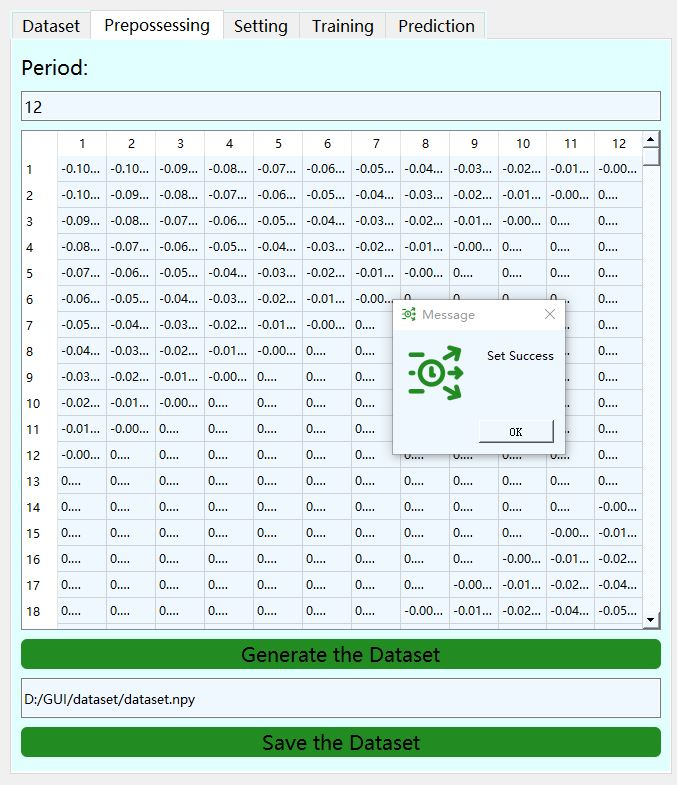
\includegraphics[width = 0.48\textwidth]{figure//deal_6.jpg}\label{deal_6} 
	}\\
	\caption{数据处理模块操作}
	\label{deal}
\end{figure}

\begin{itemize}
	\item 序列周期输入框:时间序列周期(period)输入框由QLineEdit组件实现。该组件用来存放时间序列的周期,数据类型为整型,且不能为0,如图\ref{deal_2}。
	\item 数据集处理按钮:数据集处理按钮由QPushButton组件实现。单击按钮后,根据周期长度生成行为样本个数,列为周期长度的数据表组件QTableWidget,如图\ref{deal_3}。
	\item 时间序列数据表:数据表由QTableWidget组件实现。用来存放处理后的时间序列预测数据集,行为样本个数,列为周期长度,数据表中的值为浮点型小数,表的行数和列数会根据数据行列的变化而变化,表格中的数据不可编辑,如图\ref{deal_3}。
	\item 数据表保存按钮:数据表保存按钮由QPushButton组件实现。单击按钮后,弹出数据保存框,数据是ndarray格式的数据类型,数据必须保存在项目根目录的dataset文件夹下,为的是以后训练时方便读取,单击保存框的保存按钮ndarray格式的数据会通过joblib的save方法以npy格式的压缩文件存储在本地磁盘,如图\ref{deal_4}和图\ref{deal_5}。
	\item 保存路径显示框:路径显示框由QLineEdit组件实现。数据保存后的路径会显示在该文本框中,如图\ref{deal_6}。
\end{itemize}

\section{参数设置模块}

参数设置模块使用网格布局QGridLayout,它的整体是一个QWidget窗口组件,宽高均为自适应。该模块由五个部分组成,分别是模糊集个数输入框,模糊系统层数输入框,卷积操作滑窗长度输入框,滑窗步长输入框和参数保存按钮,如图\ref{set_1}。其中四个输入框均可以编辑,每个输入框都有默认值,模糊集个数默认值为20,模糊系统层数默认值为5,卷积操作滑窗长度默认值为3,滑窗步长默认值为1,按钮可重复单击,如图\ref{set_2}。

\begin{figure}
	\centering
	\subfigure[参数设置模块]{
		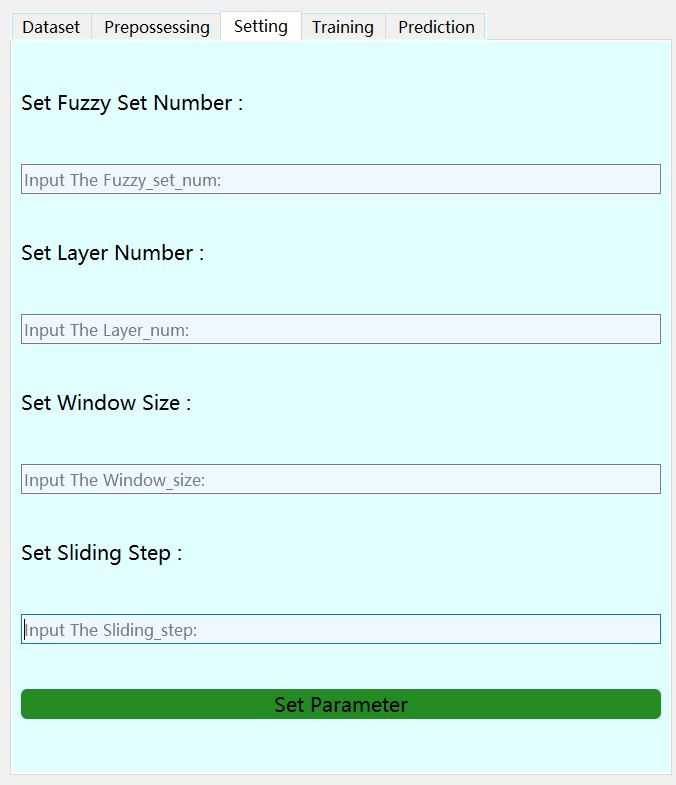
\includegraphics[width = 0.48\textwidth]{figure//set_1.jpg}\label{set_1}
	}
	\subfigure[参数输入操作]{
		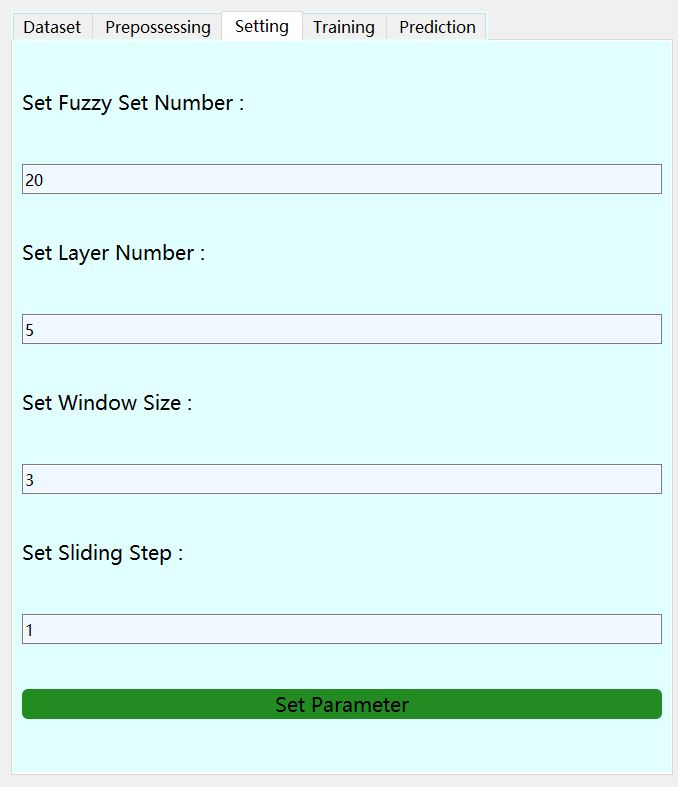
\includegraphics[width = 0.48\textwidth]{figure//set_2.jpg}\label{set_2} 
	}
	\subfigure[参数保存成功操作]{
		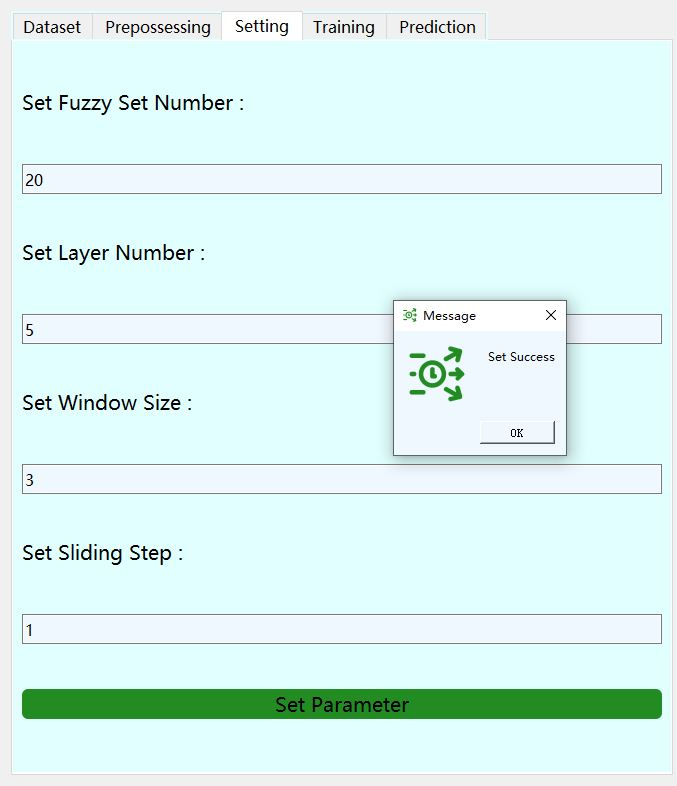
\includegraphics[width = 0.48\textwidth]{figure//set_3.jpg}\label{set_3} 
	}
	\subfigure[参数保存失败操作]{
		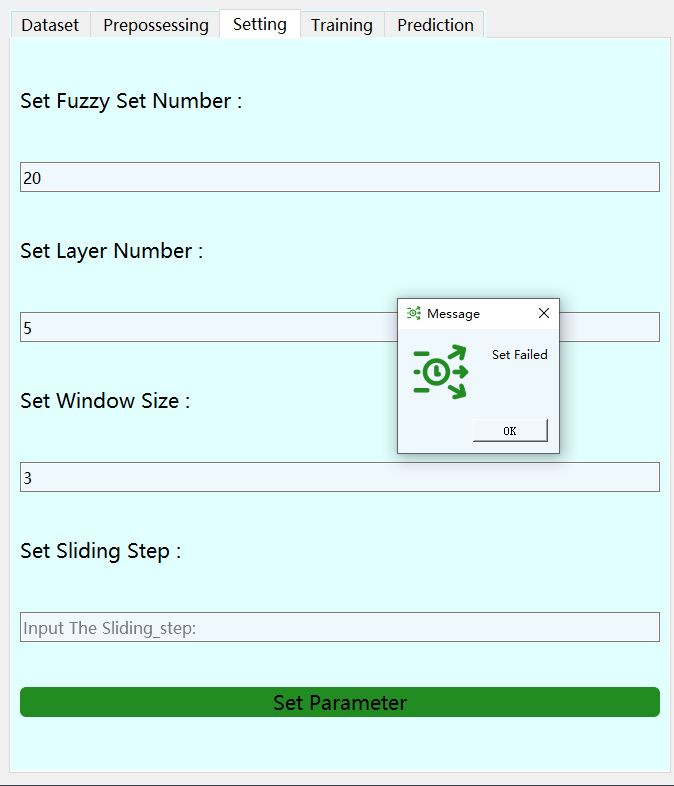
\includegraphics[width = 0.48\textwidth]{figure//set_4.jpg}\label{set_4} 
	}\\
	\caption{参数设置模块操作}
	\label{set}
\end{figure}

\begin{itemize}
	\item 模糊集个数输入框:模糊集个数(fuzzy set number)输入框由QLineEdit组件实现。
	\item 模糊系统层数输入框:模糊系统层数(layer number)输入框由QLineEdit组件实现。
	\item 卷积操作滑窗长度输入框:卷积操作滑窗长度(window size)输入框由QLineEdit组件实现。
	\item 滑窗步长输入框:滑窗步长(sliding step)输入框由QLineEdit组件实现。
	\item 参数设置按钮: 参数保存按钮由QPushButton组件实现。单击设置按钮后,四个参数先存入一个1维的array数组,再以npy格式的数据文件保存在项目根目录的parameter文件夹下。若四个参数都不为空值,参数保存成功后弹出“Set Success”的消息提示框,如图\ref{set_3},若其中至少有一个文本框未设置参数,则弹出“Set Failed”消息提示框,如图\ref{set_4}。提示框由QMessageBox组件实现,这里选用的时QMessageBox的关于对话框(about),关于对话框只有一个按钮,对点击的按钮所响应的事件确认,显示的消息是对当前操作的结果进行描述,如“Set Success”,“Set Failed”。
\end{itemize}

\section{模型训练模块}

模型训练模块使用网格布局QGridLayout,它的整体是一个QWidget窗口组件,宽高均为自适应。该模块由三个部分组成,训练集测试结果显示框,训练集测试结果作图展示框,模型训练按钮,按钮可重复单击。

\begin{figure}
	\centering
	\subfigure[模型训练模块]{
		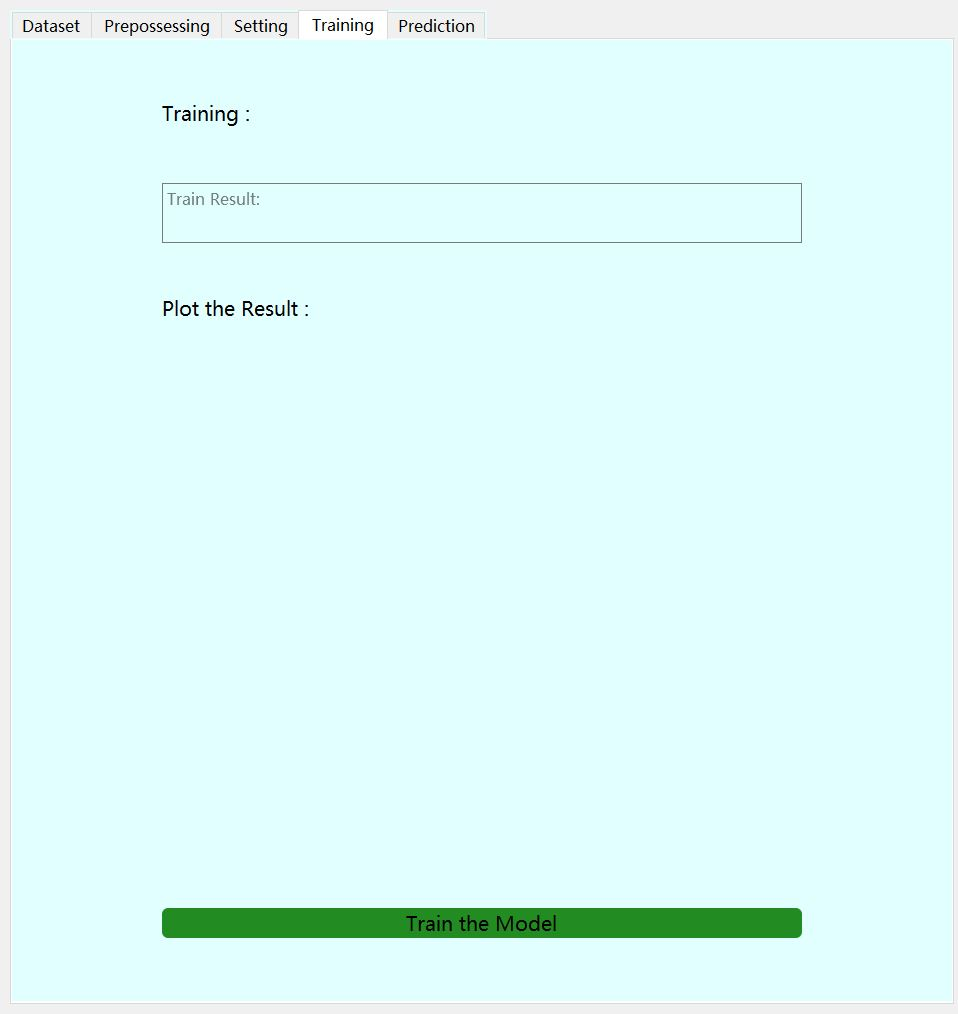
\includegraphics[width = 0.48\textwidth]{figure//train_1.jpg}\label{train_1}
	}
	\subfigure[训练过程控制台]{
		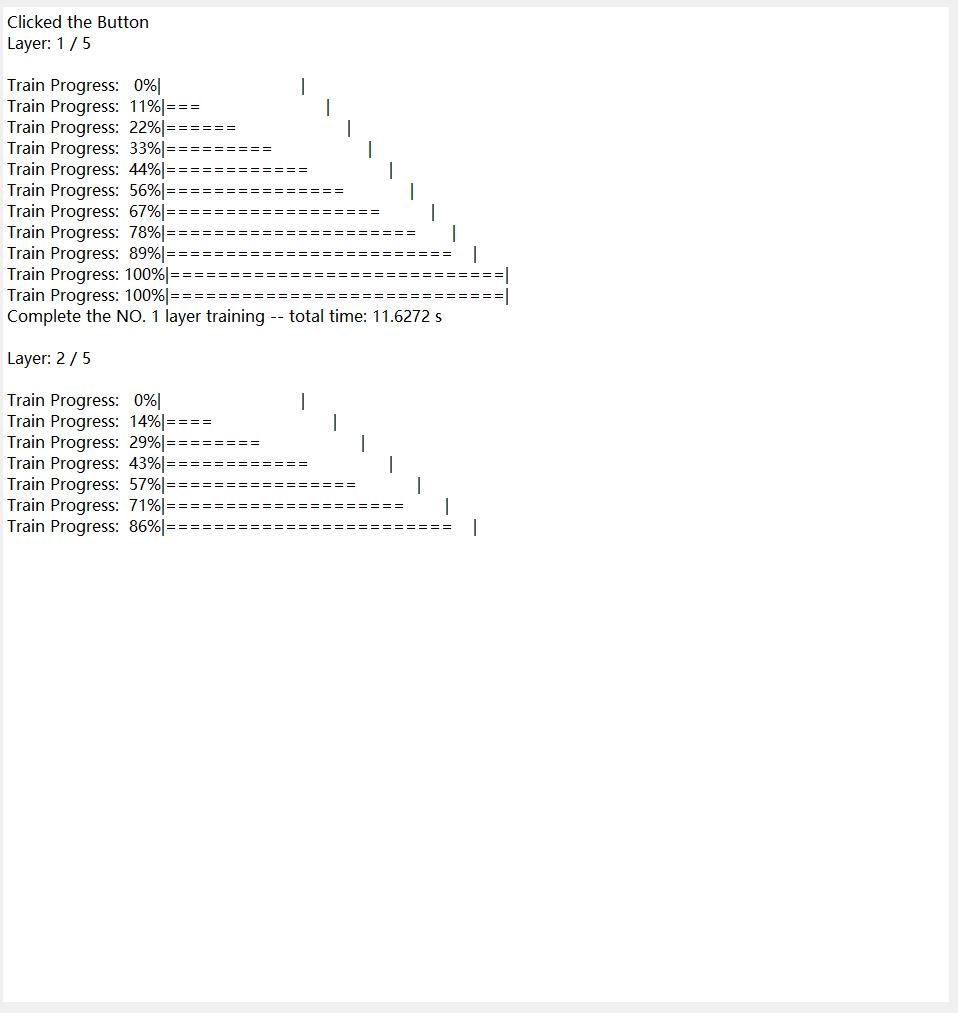
\includegraphics[width = 0.48\textwidth]{figure//train_2.jpg}\label{train_2} 
	}
	\subfigure[模型训练结束]{
		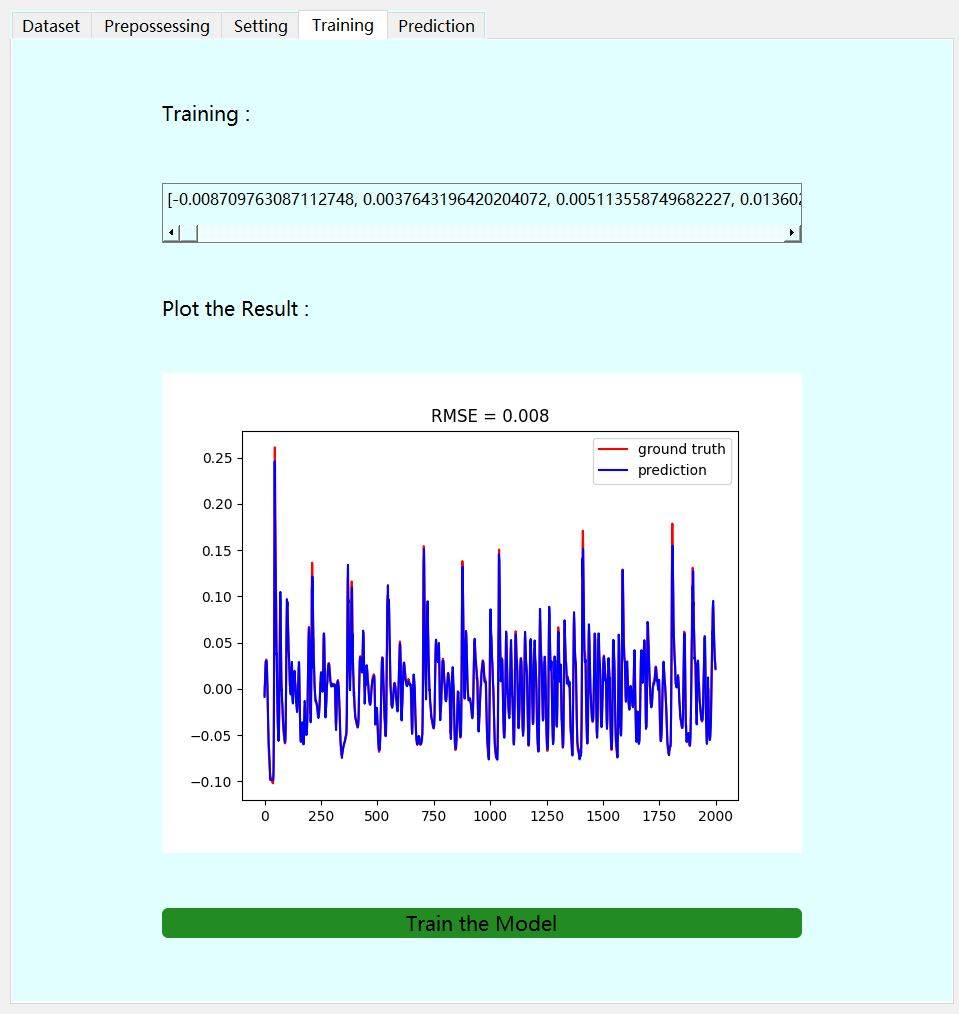
\includegraphics[width = 0.48\textwidth]{figure//train_3.jpg}\label{train_3} 
	}
	\subfigure[训练结束控制台]{
		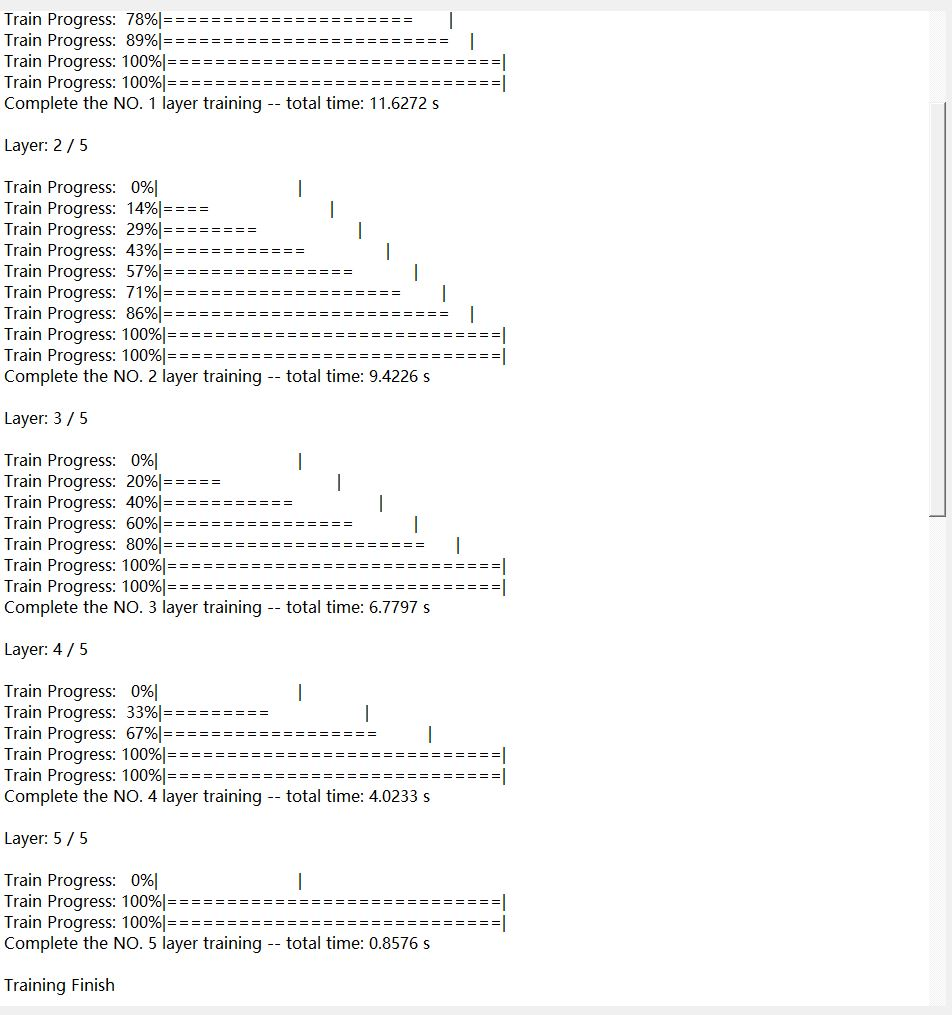
\includegraphics[width = 0.48\textwidth]{figure//train_4.jpg}\label{train_4} 
	}\\
	\caption{模型训练模块操作}
	\label{train}
\end{figure}

\begin{itemize}
	\item 训练集测试结果显示框:
	\item 训练集测试结果作图展示框:
	\item 模型训练按钮:
\end{itemize}

\section{模型预测模块}

模型预测模块使用网格布局QGridLayout,它的整体是一个QWidget窗口组件,宽高均为自适应。该模块由三个部分组成,测试集结果显示框,预测结果作图展示框,模型预测按钮,按钮可重复单击。

\begin{figure}
	\centering
	\subfigure[模型预测模块]{
		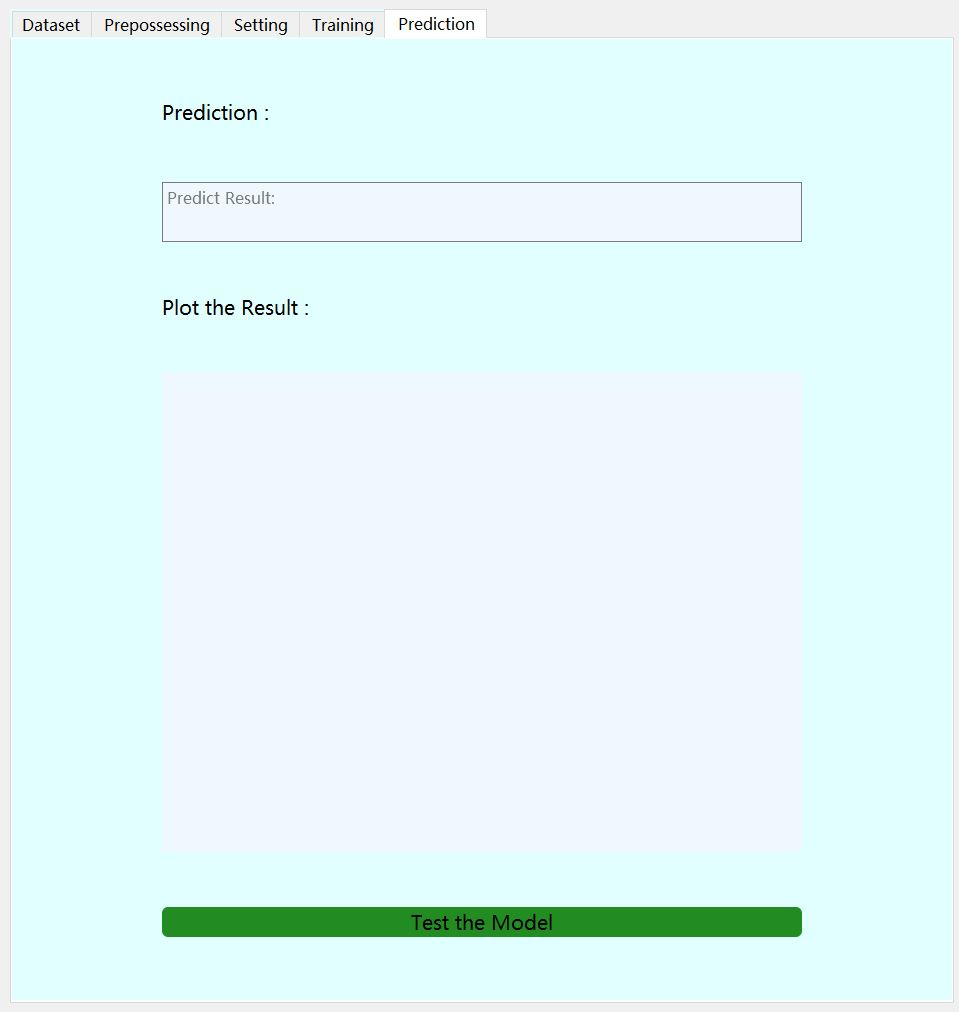
\includegraphics[width = 0.48\textwidth]{figure//test_1.jpg}\label{test_1}
	}
	\subfigure[预测过程控制台]{
		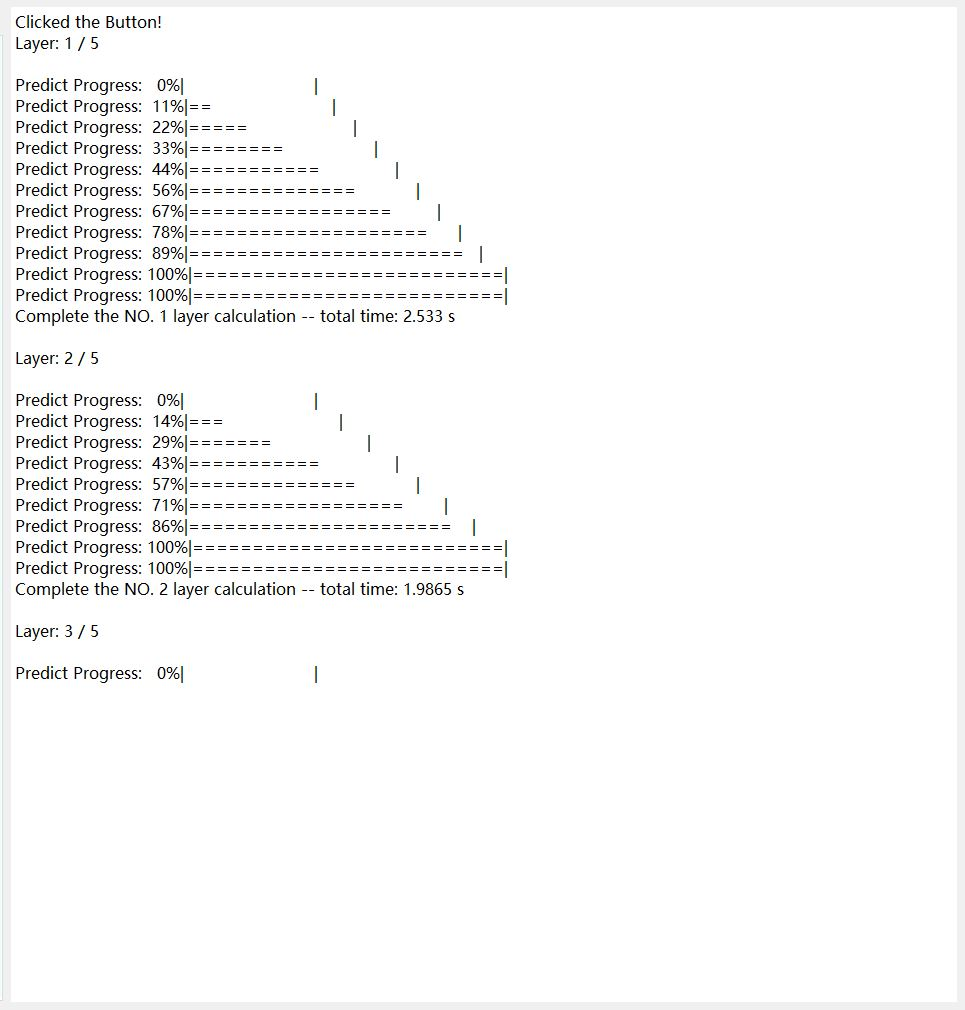
\includegraphics[width = 0.48\textwidth]{figure//test_2.jpg}\label{test_2} 
	}
	\subfigure[模型预测结束]{
		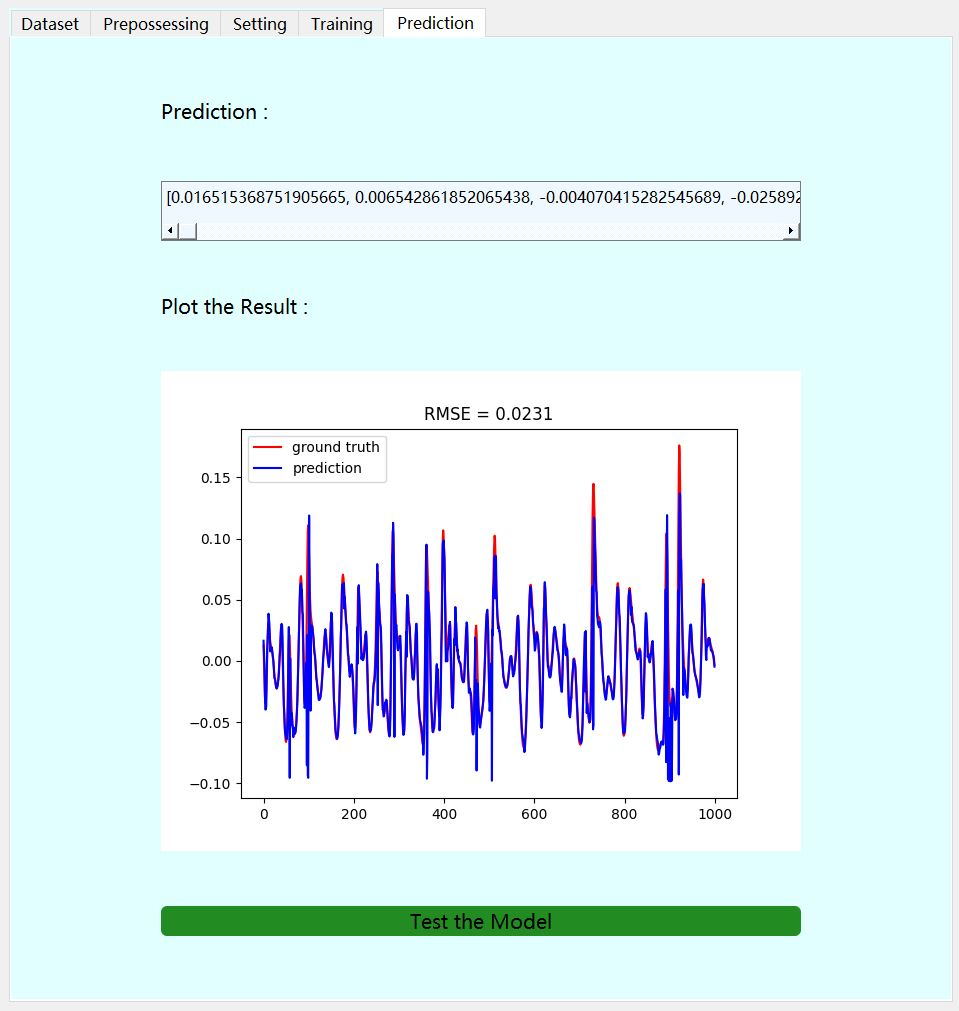
\includegraphics[width = 0.48\textwidth]{figure//test_3.jpg}\label{test_3} 
	}
	\subfigure[预测结束控制台]{
		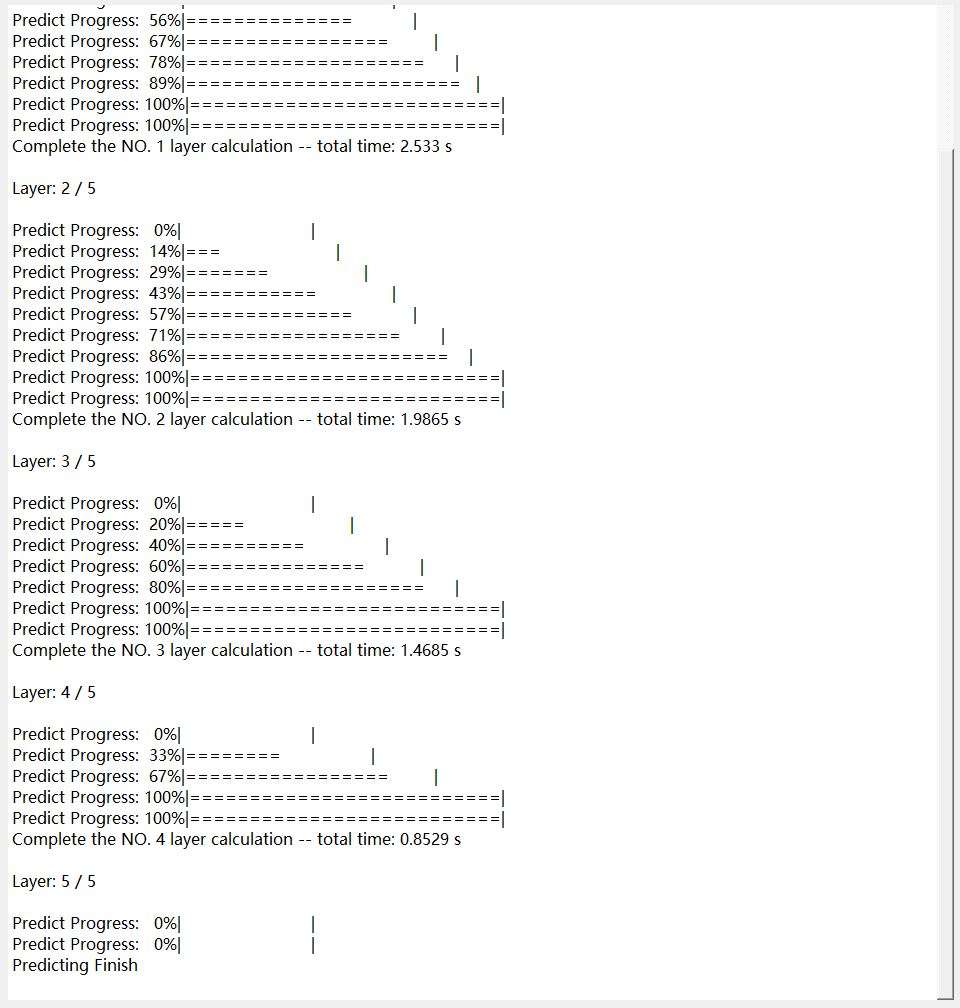
\includegraphics[width = 0.48\textwidth]{figure//test_4.jpg}\label{test_4} 
	}\\
	\caption{模型预测模块操作}
	\label{test}
\end{figure}

\begin{itemize}
	\item 预测结果显示框:
	\item 预测结果作图展示框:
	\item 模型预测按钮:
\end{itemize}

\chapter{平台操作流程}

\end{document}
